% DSA4212 group project report: Muon's late-training update under gradient noise.
% Build: pdflatex main; bibtex main; pdflatex main; pdflatex main   (or upload report/ to Overleaf).
% Limit: 10 pages INCLUDING references and appendix. Names, student numbers and the GitHub URL on page 1.
% No code in the main text. The plan, page budget and verified numbers are in report/outline.md.
% Every number comes from results/ or notes/lab_notebook.md. Figures: code/plot_report.py (and
% code/plot_e3.py for Figure A1); tables 2 and A1: code/make_tables.py. Label exploratory results in the
% text and in their captions. Page budgets assume about 550 words of text per full page.

\documentclass[11pt,a4paper]{article}
\usepackage[margin=2.5cm]{geometry}
\usepackage[T1]{fontenc}
\usepackage{lmodern}
\usepackage{microtype}
\usepackage{amsmath,amssymb}
\usepackage{graphicx}
\usepackage{booktabs}
\usepackage[font=small,labelfont=bf]{caption}
\usepackage[round,authoryear]{natbib}
\usepackage{xcolor}
\usepackage[hidelinks]{hyperref}
\graphicspath{{figures/}}
\newcommand{\todo}[1]{\textcolor{red}{[TODO: #1]}}  % none may remain at submission

\title{Flatten More, Not Less: Muon's Late-Training Update under Gradient Noise}  % working title
\author{%
  Chee Jia Yun (\todo{student number}) \and
  \todo{member 2 (student number)} \and
  \todo{member 3 (student number)} \and
  \todo{member 4 (student number)}\\[6pt]
  \normalsize Code, configs and results: \url{https://github.com/jiayunchee/dsa4212_Muon}}
\date{DSA4212 \quad \todo{submission date}}

\begin{document}
\maketitle

% ---- Title block and abstract: 0.4 page. Abstract about 150 words. ----
\begin{abstract}
\todo{About 150 words: the question; the setup in one sentence; the four story sentences of the outline,
compressed; one line saying which results are exploratory.}
\end{abstract}

% =====================================================================================================
\section{Introduction}\label{sec:intro}
% Budget: 0.7 page, about 380 words, no figures.
% Takeaway: the question is open, and it can be tested here.
% - Muon flattens the singular values of each hidden-layer update. The brief asks whether boosting weak
%   directions helps, or amplifies noise.
% - Late training: Xie (2026) says switch to momentum SGD when noise dominates; DynMuon (Wu et al., 2026)
%   says flatten even more (p = -0.25).
% - Our question: does the best late-phase exponent p in U S^p V^T depend on gradient noise?
% - Contributions (3 bullets): fairly tuned per-step and per-second baselines; a pre-registered branch
%   test over 8 noise conditions; an exploratory follow-up that brackets p*.
\todo{Write.}

% =====================================================================================================
\section{Background}\label{sec:background}
% Budget: 0.8 page, about 440 words.
% Takeaway: what p means, and what each theory predicts.
% - The Muon update: EMA momentum, the Nesterov input N, Newton-Schulz ~ polar factor U V^T, the shape
%   factor sqrt(max(1, m/n)). Equation (1) below gives the family studied.
% - p = 0 is exact Muon, p = 1 normalised momentum SGD, p < 0 boosts weak directions further.
% - Xie's indicator delta (signal over noise, per layer) and the matched switch; DynMuon's late p = -0.25.
% - Why step sizes must be tuned per p: Shumaylov et al. (2026). READ BEFORE CITING (abstract only).
For a hidden weight matrix $W \in \mathbb{R}^{m \times n}$ with Nesterov momentum input
$N = U S V^\top$ (thin SVD, numerical rank $r$), we study the update family
\begin{equation}
  D_p = \frac{\sqrt{r}}{\lVert U S^{p} V^\top \rVert_F}\; U S^{p} V^\top ,
  \qquad
  W \leftarrow W - \eta \sqrt{\max(1, m/n)}\; D_p .
  \label{eq:family}
\end{equation}
\todo{Write the rest.}

% =====================================================================================================
\section{Setup and protocol}\label{sec:setup}
% Budget: 1.5 pages including Table 1 (about 0.2 page): about 700 words.
% Takeaway: the comparison is fair, and the brief's three rules are met:
%   (R1) same models and data, comparable tuning, stated budgets; (R2) per step and per time reported
%   separately; (R3) which parameters get Muon.
% - Task A: teacher-student regression with a fresh minibatch every step; input covariance with
%   eigenvalues ~ 1/i; label noise sigma_y = 0.5. Excess risk against the noiseless teacher on 16,384
%   fixed inputs, so the optimum is known.
% - Student: tanh MLP 128-256-256-256-16. (R3) Only the two 256 x 256 hidden matrices get the Muon
%   family; the first and last layers and the biases use AdamW at E1's best rate for that B.
% - Branch design: exact Muon for 3000 steps (E2, 5 seeds); every arm continues from the same checkpoint
%   with the same future data, so comparisons are paired.
% - (R1) Tuning: E1, 5 learning rates per optimiser and B. E3/F1, a multiplier per arm from {0.5, 1, 2},
%   extended by halving or doubling while the best is on an edge, within [1/64, 64]. Tuning seeds
%   {0, 1}; evaluation seeds {2, 3, 4}.
% - Statistics: paired 95% t-intervals against p = 0; p* with a bootstrap over seeds; the H1 contrast C.
% - Pre-registration: protocol fixed 20 Oct; a dated change log records the extension rule, the stopping
%   rule, the frozen control, F1 and the timing benchmark.
% - Budget: 1179 training runs, all on one CPU in float32 (bf16 is about 200-400x slower on this CPU).
\todo{Write.}

\begin{table}[t]
  \centering
  \caption{The experiments. Tuning and evaluation use separate seeds; all runs are on one CPU in float32.}
  \label{tab:experiments}
  \small
  \begin{tabular}{@{}lp{6.4cm}rll@{}}
    \toprule
         & Purpose                                                              & Runs              & Seeds        & Status         \\
    \midrule
    E0   & Pilot: timing and learning-rate ranges                               & 16                & 0            & pilot          \\
    E1   & Baselines, learning rate tuned per optimiser and batch size          & 164               & 0, 1         & pre-registered \\
    E2   & Shared exact-Muon phase (3000 steps), checkpoints                    & 40                & 0--4         & pre-registered \\
    E3   & Branches $p \in \{-0.25, 0, 0.5, 1\}$, NS5, Xie: tuning / evaluation & 470 / 144         & 0, 1 / 2--4  & pre-registered \\
    E3c  & Branches with the hidden layers frozen                               & 40                & 0--4         & exploratory    \\
    F1   & Branches $p \in \{-0.75, -0.5\}$: tuning / evaluation                & 212 / 48$^{a}$    & 0, 1 / 2--4  & exploratory    \\
    E-T  & Time per step, median of 5 passes                                    & --                & --           & pre-registered$^{b}$ \\
    \bottomrule
  \end{tabular}

  \smallskip
  \footnotesize $^{a}$Plus 45 superseded runs at a step size selected before tuning had finished; kept,
  not used. $^{b}$Changed on 28 Oct from one pass to the median of 5 passes (protocol change log).
\end{table}

% =====================================================================================================
\section{Muon against the baselines, per step and per second}\label{sec:baselines}
% Budget: 1.2 pages including Figure 1 (about 0.35 page): about 450 words.
% Takeaway: Muon wins per step and mostly loses per second here, and why. (R2)
% Numbers (verified, see the outline):
% - Per step: exact Muon is 37.5 / 25.2 / 29.1 / 45.1% below the better baseline (SGD each time) at
%   B = 16 / 64 / 256 / 1024; NS5 ~ exact Muon (-0.2% to +2.4%).
% - Best learning rates: from B = 16 to 1024, SGD's rises 10x and AdamW's 3x; Muon's falls 0.003 -> 0.001.
% - Per second (median of 5 benchmark passes): Muon's overhead over SGD is 2.0-3.2 ms per step (NS5) and
%   7.9-9.5 ms (exact SVD). At SGD's 6000-step time, SGD wins at B <= 256 (NS5 has 1.3-2.9x SGD's
%   excess risk); NS5 wins at B = 1024 (0.0058 vs 0.0079). Same winner under all three timing sets;
%   NS5's lead at B = 1024 is 10-27%.
% - One sentence on the pilot: its reversed ranking came from untuned Muon learning rates.
% - Caution: the timings are CPU-specific and vary with machine load.
\todo{Write.}

\begin{figure}[t]
  \centering
  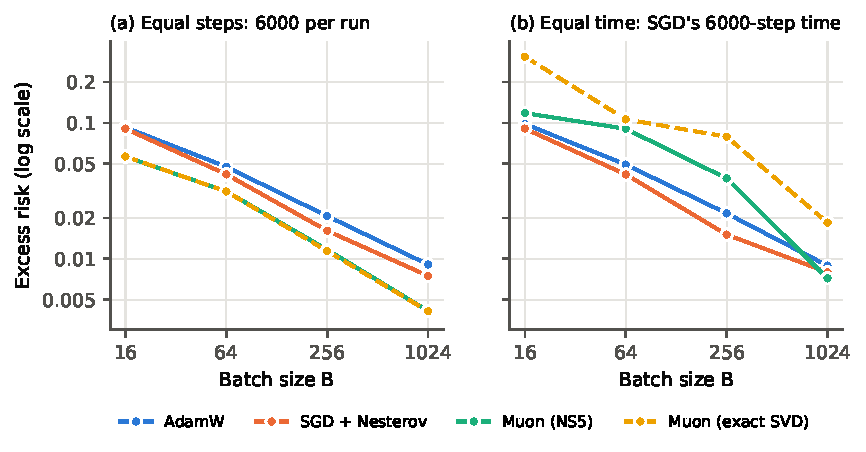
\includegraphics[width=\linewidth]{fig1_step_vs_time}
  \caption{Tuned baselines on Task~A, per step and per second. (a)~Tail excess risk (mean over the last
  10\% of 6000 steps, mean of 2 seeds) at each optimiser's best learning rate. (b)~Excess risk at equal
  wall-clock time: the seed-averaged curve read at the time SGD needs for 6000 steps, with the median
  time per step over 5 benchmark passes (one CPU thread). The shared log axis shows the cost of Muon's
  slower steps: per step, both Muons lead at every batch size; per second, only NS5 Muon beats SGD, and
  only at $B=1024$.}
  \label{fig:baselines}
\end{figure}

% =====================================================================================================
\section{Pre-registered test: the late-phase exponent under noise}\label{sec:e3}
% Budget: 1.5 pages including Figure 2 and Table 2 (about 0.6 page together): about 480 words.
% Takeaway: flattening more wins everywhere; H1 and H2 fail as stated.
% - Noise at the switch: delta from 0.69 (B = 16, beta = 0.9) to 4.09 (B = 1024, beta = 0.95); only one
%   condition is clearly noise-dominated (Table 2, Figure A1).
% - Changes against continuing Muon (evaluation seeds): p = -0.25 -2.4 to -7.6%; p = 0.5 +8.6 to +21.2%;
%   p = 1 +11.7 to +41.5%; Xie +11.8 to +37.4%; NS5 -1.3 to +1.7%. p* = -0.25 in all 8 conditions.
% - Verdicts: H1 contradicted, C = +0.00877 [+0.00833, +0.00922] (beta 0.9) and +0.00657 [+0.00617,
%   +0.00698] (beta 0.95); H2 not supported; H3 not testable (p* constant).
% - Disclose the design flaw: C compares absolute gaps, and excess risk is about 14x larger at B = 16.
\todo{Write.}

\begin{figure}[t]
  \centering
  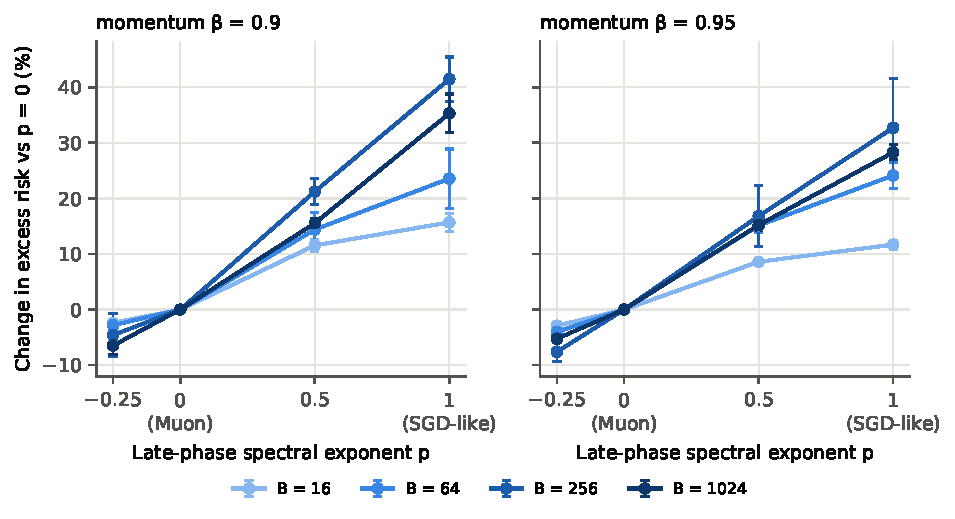
\includegraphics[width=\linewidth]{fig2_e3_relative_change}
  \caption{Pre-registered test (E3). Change in tail excess risk when training continues from the same
  Muon checkpoint with spectral exponent $p$ instead of Muon ($p=0$), each arm at its own tuned step
  size. Mean and 95\% $t$-interval over 3 evaluation seeds; below 0 is better than continuing Muon. In
  every condition $p=-0.25$ is best and the SGD-like end ($p=1$) is worst.}
  \label{fig:e3}
\end{figure}

\begin{table}[t]
  \centering
  \caption{Per condition: Xie's noise indicator $\delta$ at the switch; the best exponent among those
  tested (E3: pre-registered; F1: exploratory, adds $p=-0.5$ and $p=-0.75$); and the change in tail
  excess risk against continuing Muon, mean over 3 evaluation seeds.}
  \label{tab:conditions}
  \small
  \begin{tabular}{@{}rrrrrrrr@{}}
\toprule
 & & & \multicolumn{2}{c}{Best $p$} & \multicolumn{3}{c}{Change vs.\ Muon (\%)} \\
\cmidrule(lr){4-5}\cmidrule(l){6-8}
$B$ & $\beta$ & $\delta$ & E3 & F1 & $p=-0.25$ & $p=1$ & Xie \\
\midrule
16 & 0.9 & 0.69 & $-0.25$ & $-0.25$ & $-2.4$ & $+15.7$ & $+15.6$ \\
16 & 0.95 & 1.10 & $-0.25$ & $-0.25$ & $-2.9$ & $+11.7$ & $+11.8$ \\
64 & 0.9 & 1.16 & $-0.25$ & $-0.25$ & $-2.8$ & $+23.6$ & $+23.5$ \\
64 & 0.95 & 1.84 & $-0.25$ & $-0.25$ & $-4.0$ & $+24.1$ & $+23.7$ \\
256 & 0.9 & 1.77 & $-0.25$ & $-0.5$ & $-4.6$ & $+41.5$ & $+37.4$ \\
256 & 0.95 & 2.76 & $-0.25$ & $-0.5$ & $-7.6$ & $+32.7$ & $+31.2$ \\
1024 & 0.9 & 2.62 & $-0.25$ & $-0.5$ & $-6.5$ & $+35.3$ & $+33.2$ \\
1024 & 0.95 & 4.09 & $-0.25$ & $-0.5$ & $-5.2$ & $+28.3$ & $+28.3$ \\
\bottomrule
\end{tabular}

\end{table}

% =====================================================================================================
\section{Exploratory follow-ups}\label{sec:exploratory}
% Budget: 1.1 pages including Figure 3 (about 0.35 page): about 400 words.
% Takeaway: the optimum shifts mildly with batch size, and the SGD-like arms lose for an identifiable
% reason. Say once at the top, and in every caption, that this section is exploratory.
% - F1: p* = -0.25 at B <= 64 and -0.5 at B >= 256, both beta. p = -0.5 minus p = -0.25: +1.4 to +4.1%
%   at B <= 64, -1.3 to -2.4% at B >= 256; 7 of 8 intervals exclude 0. rho(delta, p*) = -0.76 (exact
%   permutation p = 0.029); rho(log B, p*) = -0.89; momentum changes delta by 56-60% without moving p*.
%   The new arms needed x8-x32 at B >= 64; at x2, p = -0.5 looked up to 43% worse than Muon.
% - Frozen control: at B = 16 the SGD-like arms are no better than freezing the hidden layers (p = 1:
%   0.0672 vs 0.0675 at beta = 0.9); at B = 1024 they clearly beat it (0.0056 vs 0.0076).
% - Scale-free contrast: -0.199 and -0.163 (H1's direction); the gain of p = -0.25 over Muon rises with
%   delta (rho = +0.88).
\todo{Write.}

\begin{figure}[t]
  \centering
  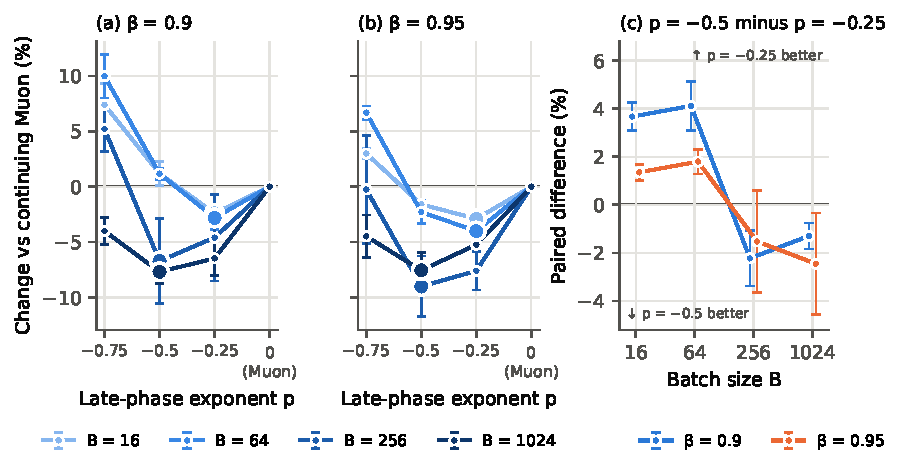
\includegraphics[width=\linewidth]{fig3_f1_exponent_shift}
  \caption{Exploratory follow-up F1 (not pre-registered). (a,~b)~As Figure~\ref{fig:e3}, for $p \le 0$,
  including the added arms $p=-0.5$ and $p=-0.75$; each batch size's best $p$ is drawn larger.
  (c)~Paired difference between $p=-0.5$ and $p=-0.25$, in \% of the excess risk at $p=-0.25$; mean and
  95\% $t$-interval over 3 seeds. Below 0, flattening more is better; the sign flips between $B=64$
  and $B=256$.}
  \label{fig:f1}
\end{figure}

% =====================================================================================================
\section{Discussion and limitations}\label{sec:discussion}
% Budget: 0.9 page, about 500 words.
% Takeaway: what this means for using Muon, and how far it generalises.
% - Against the two theories: DynMuon's mildly negative p holds across a 64x range of batch size; Xie's
%   regime (delta << 1 near the optimum) was never reached (smallest delta 0.69).
% - Why SGD-like steps fail at small batch (frozen control). Hypothesis, labelled as such: the
%   hidden-layer gradients are ill-conditioned, so a step large enough for the weak directions is too
%   large for the strong ones.
% - Step size and shape are coupled: more negative p needs larger multipliers; this decided both the
%   pilot and F1.
% - Limitations: one synthetic task and a small MLP; CPU float32, not bf16; weight decay 0; 3 evaluation
%   seeds; p grid in steps of 0.25; equal steps across B (larger batches see more data); timing is
%   hardware- and load-dependent; F1 not pre-registered. Without E5, H2 is "not supported in our noise
%   regime", not "refuted".
\todo{Write.}

\section{Conclusion}\label{sec:conclusion}
% Budget: 0.2 page, about 110 words. Three lines: the main answer, the exploratory refinement, the
% method lesson (per-arm step-size tuning decided every answer).
\todo{Write.}

% ---- References: about 0.5 page. Cite a source only for claims in parts we have read
% (notes/reading_list.md); references.bib marks the entries still to read. ----
\nocite{*}  % TODO: remove once the text cites; for now it lists every entry so the length shows
\bibliographystyle{plainnat}
\bibliography{references}

% =====================================================================================================
\appendix
\section{Additional details}\label{app:details}
% Budget: 0.7 page in total, including Table A1 and Figure A1.
% - Extension rounds: edge cells 37 -> 7 -> 3 -> 0 (E3) and 16 -> 12 -> 2 -> 0 (F1).
% - Implementation checks: 26 unit tests; MinimalMuon matches torch.optim.Muon exactly; float64 SVD
%   retries are counted in every run.
% - Deviations from the protocol: one line per dated change-log entry.
% - Reproduction: point to the README table; no commands here.
\todo{Write.}

\begin{table}[h]
  \centering
  \caption{Selected step-size multiplier of every arm in every condition, chosen on tuning seeds 0 and 1.
  It scales the learning rate at the switch (exact Muon's tuned E1 rate) or, for Xie's switch, Xie's
  matched momentum-SGD rate.}
  \label{tab:multipliers}
  \small
  \begin{tabular}{@{}rrrrrrrrrr@{}}
\toprule
 & & \multicolumn{6}{c}{Spectral exponent $p$} & & \\
\cmidrule(lr){3-8}
$B$ & $\beta$ & $-0.75$ & $-0.5$ & $-0.25$ & 0 & 0.5 & 1 & NS5 & Xie \\
\midrule
16 & 0.9 & 4 & 4 & 2 & 1 & 1/4 & 1/32 & 1 & 1/16 \\
16 & 0.95 & 4 & 2 & 1 & 1/2 & 1/8 & 1/32 & 1/2 & 1/32 \\
64 & 0.9 & 16 & 8 & 8 & 2 & 1 & 1/2 & 4 & 1 \\
64 & 0.95 & 16 & 8 & 4 & 2 & 1/2 & 1/4 & 2 & 1/2 \\
256 & 0.9 & 32 & 16 & 8 & 2 & 2 & 2 & 4 & 2 \\
256 & 0.95 & 16 & 8 & 4 & 2 & 1/2 & 1/2 & 2 & 1 \\
1024 & 0.9 & 32 & 16 & 4 & 2 & 1 & 1 & 2 & 2 \\
1024 & 0.95 & 16 & 8 & 2 & 1 & 1/2 & 1/2 & 1 & 1 \\
\bottomrule
\end{tabular}

\end{table}

\begin{figure}[h]
  \centering
  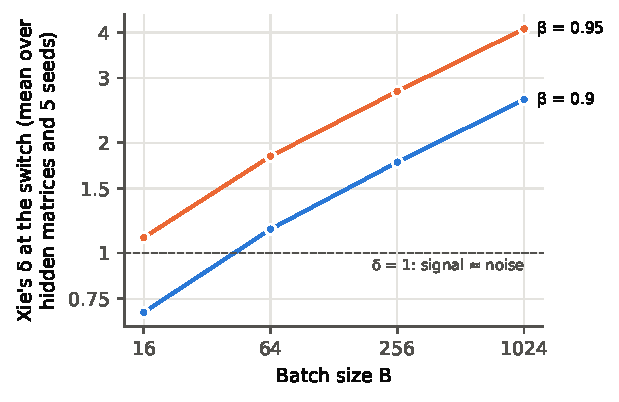
\includegraphics[width=0.55\linewidth]{e4_delta_vs_batch}
  \caption{Xie's noise indicator $\delta$ at the switch (step 3000), mean over both hidden matrices and
  5 seeds. Below 1, noise dominates the momentum.}
  \label{fig:delta}
\end{figure}

\end{document}
